\chapter{Introducao}
\label{cap:introduction}

THYAGO vai fazer a parte introdut�ria at� as tecnologias.
Ele ja sabe o que fazer.

\section{Hist�ria}
\label{sec:history}
Thyago

\section{Objetivos}
\label{sec:obj}
Thyago
\section{Metodologia}
\label{sec:methodology}
Thyago
\chapter{Tecnologia de Transporte}
\label{cap:technology}
FABIO faz a parte de Tecnologias 
e Isaac faz a parte de multiplexa��o dessas tecnologias.

\section{PDH}
\label{sec:pdh}
PDH VAI FICAR AQUI OU VAI SER FALADO SOMENTE NO HIST�RICO?

\section{SONET e SDH}
\label{sec:sdh}

A tecnologia de transporte PDH, que foi introduzida para atender a demanda de multiplexa��o de canais de voz, apresentava uma s�rie de limita��es tecnol�gicas e operacionais, o que fez com que na d�cada de 1980 fornecedores de servi�os de telecomunica��es e fabricantes de equipamentos buscassem novos padr�es de transmiss�o e multiplexa��o, com foco na transmiss�o �ptica. Em 1984, a associa��o americana chamada \ac{ECSA} iniciou trabalhos com a finalidade de desenvolvimento de um padr�o que atendesse as necessidades das telecomunica��es essencialmente nos Estados Unidos, propondo-o ao \ac{ANSI} e no ano de 1985, j� se tinham resultados que conduziram ao in�cio da padroniza��o da tecnologia de transporte em redes de telecomunica��es chamada de \ac{SONET}~\cite{Ballart2002}, adotado em pa�ses como Estados Unidos, Canada e Jap�o. O  \ac{CCITT}, atualmente conhecido como \ac{ITU-T}, demonstrou interesse pelo padr�o \ac{ANSI}~\cite{Boehm1990} e prop�s mudan�as para a acomoda��o de ambas as hierarquias de taxas de transmiss�o americanas e europeias e finalmente em 1988 alcan�ou-se um acordo, de modo que o �rg�o CCITT definiu o padr�o conhecido como \ac{SDH}, amplamente adotado na Europa e tamb�m no Brasil. As recomenda��es ANSI T1.105, ANSI T1.106 e ANSI T1.117 s�o exemplos de publica��es que definem par�metros relacionados a SONET enquanto as recomenda��es ITU-T G.691, ITU-T G.707 e ITU-T G.781 s�o exemplos relacionados ao padr�o SDH.

SONET e SDH guardam os mesmos conceitos tecnol�gicos e as principais diferen�as se situam em certas denomina��es de par�metros e nas taxas de transmiss�o definidas nas hierarquias. Esses dois padr�es foram desenvolvidos visando a comunica��o por meio de fibras �pticas mas, por exemplo, SDH foi tamb�m utilizado em sistemas baseados em radio-frequ�ncia. Comparando estes dois padr�es com a tecnologia PDH, podem ser destacados as seguintes vantagens:

\begin{itemize}

\item {\bf Simplifica��es no processo de multiplexa��o:} Como j� visto anteriormente, o processo de retirada de sinais tribut�rios de baixas taxas de um sinal multiplexado de taxa superior � uma opera��o dif�cil na tecnologia PDH, devido ao fato de que s�o necess�rias demultiplexa��es e multiplexa��es sucessivas para se poder localizar o tribut�rio requerido, retir�-lo e ent�o remontar o frame de alta taxa. Isso acaba implicando em altos custos de instala��o da rede PDH e em baixa confiabilidade devido a quantidade de dispositivos eletr�nicos envolvidos nos n�s aos longo da rede. A estrutura de multiplexa��o s�ncrona de SONET/SDH permite significativa redu��o de complexidade e custos relacionados ao processo de extra��o e inser��o de tribut�rios em sinais multiplexados bem como aumenta a confiabilidade do sistema como um todo. Isso porque nas redes SONET/SDH, todos os n�s da rede tem clock sincronizados, de modo que as taxas de transmiss�o s�o simplesmente m�ltiplos de um valor base e n�o se � necess�rio o preenchimento de um tribut�rio com bits vazios para possibilitar a multiplexa��o, como era necess�rio na tecnologia PDH. Assim, a extra��o de um sinal tribut�rio de um sinal de alta taxa � simplificada. Esse processo � ainda mais simplificado devido a utiliza��o de um \textit{frame} que permite serem inseridas maiores informa��es sobre o \textit{payload}. O processo de inser��o de tribut�rios tamb�m se torna simplificado, j� que os sinais possuem taxas de transmiss�o muito mais precisas e pr�ximas umas das outras do que na tecnologia PDH~\cite{Ramaswami2010}.

\item{\bf Informa��es de Gerenciamento:} Os padr�es SONET e SDH oferecem maiores recursos de monitoramento, gerenciamento e controle do que est� presente nas redes PDH. Como ser� visto mais adiante, o \textit{frame} dos padr�es SONET e SDH oferecem campos espec�ficos a atividade de monitoramento e gest�o da comunica��o.

\item{\bf Interoperabilidade:} � dif�cil tratar de conceitos de telecomunica��es sem levar em considera��o um dos princ�pios b�sicos dessa �rea que � a Interoperabilidade. Anteriormente foi mencionado que isto era um problema nos sistemas PDH, pois diferentes fornecedores de equipamentos utilizavam interfaces e codifica��es distintas, dificultando a compatibilidade ao longo da rede. SONET e SDH s�o padr�es que tentam eliminar este problema por meio da defini��o de par�metros padr�es, como as interfaces.

\item{\bf Disponibilidade da rede:} SONET e SDH s�o padr�es que evolu�ram para acomodar espec�ficas topologias de rede e t�cnicas de prote��o e protocolos associados para possibilitar altos n�veis de disponibilidade. Como consequ�ncia, a atua��o da prote��o � em geral mais r�pida do que nas redes PDH. 


\end{itemize} 

A seguir, ser�o abordadas caracter�sticas importantes referentes a SDH. Por�m, os conceitos tamb�m se aplicam ao padr�o SONET, visto que SDH foi desenvolvido a partir do mesmo.

\subsection{Estrutura do \textit{frame} SDH}

Uma das principais caracter�sticas do \textit{frame} SDH � sua bidimensionalidade, j� que tal \textit{frame} � definido por uma quantidade de linhas e colunas como ilustrado na Figura~\ref{fig:FrameSDH}. O \textit{frame} SDH possui um n�mero fixo de linhas e um n�mero de colunas dependente da hierarquia SDH a que se est� referenciando. De forma mais precisa, tal \textit{frame} possui 9 linhas e 270 x N colunas, onde N � o termo dependente da hierarquia e que pode ser obtido observando que as hierarquias s�o definidas seguindo o padr�o \ac{STM}-N, para N igual a 1, 4, 16, 64 e 256 e � interessante ressaltar que para o caso STM-0 existem apenas 9 linhas e 90 colunas como j� indicado na Figura~\ref{fig:FrameSDH}, correspondendo ao \textit{frame} STS-1 do padr�o SONET. Cada linha nesta estrutura � tratada como um \textit{bit} enquanto cada coluna � tratada como um \textit{byte}. Outra caracter�stica importante � que independentemente do tamanho e consequentemente do n�mero de bits do \textit{frame}, sua dura��o � sempre de 125 \(\mu s\), representando uma taxa de repeti��o de 8000 kHz herdada dos antigos sistemas PDH. Nessa estrutura, os bits s�o transmitidos, da esquerda para a direita, em cada linha at� se alcan�ar o fim do \textit{frame}.

\begin{figure}[H]
 \centering
 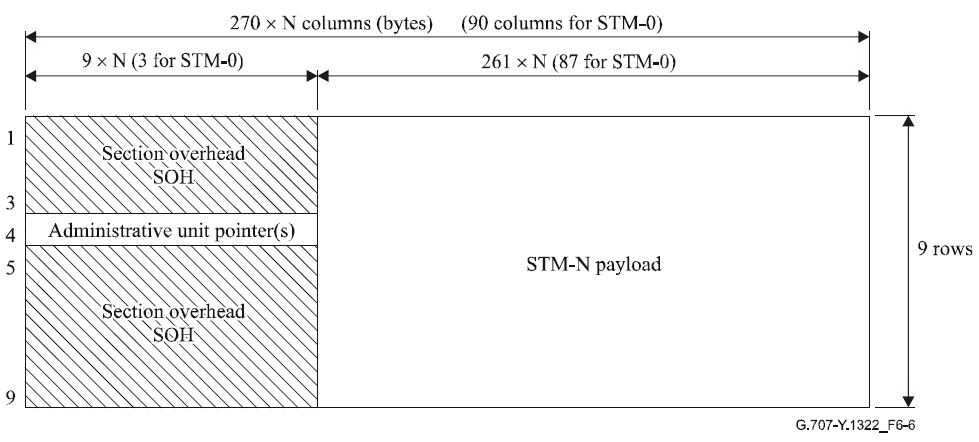
\includegraphics[scale=.6]{FrameSDH.png}
  \caption{Estrutura do \textit{frame} SDH - ITU-T G.707~\cite{G707}.}
 \label{fig:FrameSDH}
\end{figure}

O \textit{frame} SDH � formado por duas principais partes, sendo elas o cabe�alho ou \textit{overhead}, que � composto por 9 x N colunas (sendo N o n�vel da hierarquia) e 9 linhas e o \textit{payload}, composto por 261 x N colunas e 9 linhas. O \textit{payload} � a parte onde os dados dos clientes s�o inseridos para a transmiss�o. O cabe�alho, por sua vez, cont�m as informa��es do quadro \ac{STM}-N referentes a desempenho, manuten��o, monitoramento e indica��es das localidades dos tribut�rios multiplexados nos \textit{frames}, al�m de fun��es operacionais, permitindo uma ger�ncia maior por parte dos n�s da rede. Esta parte do \textit{frame} se subdivide em duas unidades b�sicas, a primeira delas sendo chamada de \ac{SOH} e a segunda de \textit{Administrative Unit Pointers}. � interessante ressaltar que \ac{SOH} ainda � separado em duas partes, sendo elas \ac{RSOH} e \ac{MSOH}, gerando a estrutura ilustrada na Figura~\ref{fig:OverheadSDH} para o cabe�alho. A seguir, apresenta-se uma breve descri��o das funcionalidade contidas em cada uma das partes mencionadas:

\begin{figure}[H]
 \centering
 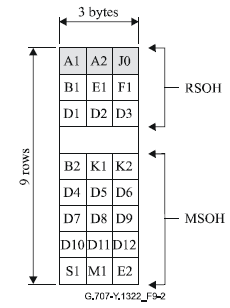
\includegraphics[scale=.7]{OverheadSDH.png}
  \caption{RSOH e MSOH - ITU-T G.707~\cite{G707}.}
 \label{fig:OverheadSDH}
\end{figure}

\begin{itemize}

\item{\bf \ac{SOH}:} Esta se��o se divide em duas partes, como indicado a seguir:

\subitem{\bf \ac{RSOH}:} Parte do cabe�alho que � processada em cada n� destinado a regenera��o. De forma mais espec�fica, essa � uma regi�o do quadro SDH que cont�m informa��es que permitem o alinhamento e identifica��o de \textit{frame}, monitoramento de erro de regenera��o, alarmes f�sicos externos ao equipamento e supervis�o de sistema.
 
\subitem{\bf \ac{MSOH}:} Parte do cabe�alho que � apenas processada em equipamentos onde existe inser��o ou retiradas de canais multiplexados. Inclui informa��es de monitoramento e indica��o de erros de multiplexa��o, controle de chaveamento de mecanismos de prote��o, monitoramento de sincronismo e ger�ncia de sistema.

\item{\bf \textit{Administrative Unit Pointers}:} Esta � uma parte do cabe�alho destinada a prover informa��es de posi��o dos dados dos clientes que foram multiplexados para formarem o \textit{frame} SDH. Possui indica��o de onde se localiza o primeiro \textit{byte} dos \ac{VC} dentro da �rea de informa��o �til (\textit{payload}) e tamb�m pode conter \textit{bytes} provenientes de justifica��o dos \ac{VC}s. � uma parte do cabe�alho processada em cada equipamento da rede

\end{itemize}

\subsection{Camadas de SDH}

A tecnologia SDH apresenta uma estrutura��o em camadas como apresentada na Figura~\ref{fig:SDHlayers}. Atrav�s de tal figura pode ser percebido que SDH possui quatro camadas, sendo elas a Camada de Via (\textit{Path layer}), Camada de Se��o de Multiplexa��o (\textit{Multiplex Section Layer}), Camada de Se��o de Regenera��o (\textit{Regeneration Section Layer}) e Camada F�sica (\textit{Physical Layer}). Para o caso das redes �pticas, a Camada F�sica diz respeito a infraestrutura �ptica de transmiss�o, com seus respectivos dispositivos~\cite{Alwayn2004}.

\begin{figure}[H]
 \centering
 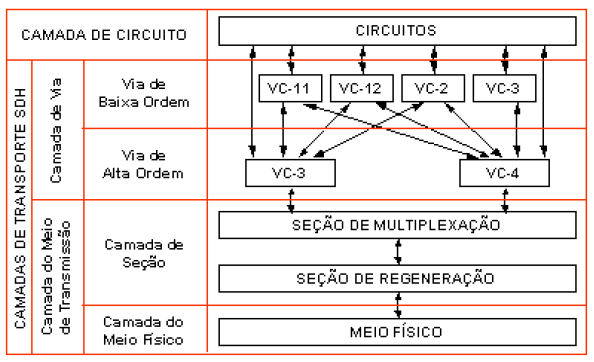
\includegraphics[scale=.7]{SDHlayers.png}
  \caption{Estrutura��o em Camadas de SDH - ~\cite{BernalFilho2003}.}
 \label{fig:SDHlayers}
\end{figure}

O conceito de via em SDH se refere a uma conex�o l�gica entre o ponto em que se monta o quadro SDH padr�o, pela inser��o de tribut�rios e o ponto em que o quadro SDH padr�o � desmontado, pela retirada de tribut�rios, ou seja, se relaciona a uma conex�o l�gica fim-a-fim. A montagem do quadro SDH consiste na a��o de inserir os dados dos clientes nas estruturas denominadas de \textit{Containers}, que consistem em unidades b�sicas de dados com bytes alocados para o transporte dos dados de mais baixas taxas dos clientes, por exemplo pode ser um sinal E1 da hierarquia PDH e associar a esses \textit{Containers} r�tulos denominados de \ac{POH} com informa��es de controle. O processo de desmontagem realiza caminho inverso, retirando o \ac{POH} e o utilizando como informa��o para dar seguimento ao conte�do dos \textit{Containers}. A Camada de Via � justamente respons�vel por realizar tais atividades e est� relacionada � conex�o fim-a-fim entre n�s SDH onde se monta e desmonta o \textit{frame}. � poss�vel que n�s intermedi�rios da rede possam realizar monitoramento de performance dos sinais da Camada de Via, por�m, os bits de cabe�alho referentes a essa camada s�o somente iniciados do ponto de montagem e terminados no ponto de desmontagem do quadro SDH.

O processo descrito anteriormente � indicado na Figura~\ref{fig:SDHlayers}, onde se indica que os dados provenientes da Camada de Circuitos s�o inseridos em \ac{VC}s. E como tamb�m pode ser analisado, a Camada de Via se divide em Via de Baixa Ordem e Via de Alta Ordem. A diferen�a b�sica entre estas duas estruturas consiste no fato de que na Via de Baixa Ordem, dados s�o inseridos em \textit{Containers} de menor tamanho e na Via de Alta Ordem, os \textit{Containers} podem carregar mais de um \ac{VC} anteriormente montado ou carregar dados de clientes que sejam de mais altas taxas de transmiss�o.














\section{OTN}
\label{sec:otn}
ALAELSON
\section{Multiplixa��o}
\label{sec:mux}
subsess�o dentro de cada tecnologia de transporte.

\section{Relacinamento entre Camadas}
\label{sec:layers}
Lailson: Est� � minha parte. Estou modificando via GIT.

\chapter{Plano de Controle}
\label{cap:control}

Alaelson

\section{GMPLS}
\label{sec:gmpls}
Alaelson
\section{SDN}
\label{sec:sdn}
Alaelslon

\chapter{Estudo de Caso: SuperComputing 2014}
\label{cap:case}
falar do chip otn da padtec
Alaelson
\chapter{Conclus�o}
\label{cap:conclusion}

Thyago